\documentclass{beamer}

\title{\yourThesisTitle}
\subtitle{\typeOfWork}
\author{\yourNameInclTitle}

\usepackage[style=apa, backend=biber, language=ngerman]{biblatex}
\addbibresource{references.bib}
\renewcommand\bibname{\section{Literaturverzeichnis}}


\usetheme{Frankfurt}
\usepackage{xcolor}

%\usepackage{textpos}
% overlay the logo on every page which is in a textblock over normal text
\usepackage[absolute,overlay]{textpos}

%\usepackage{enumitem}

\usepackage{graphicx}
\usepackage{subcaption}
\captionsetup{compatibility=false}

\definecolor{fhgreen}{rgb}{0,0.47,0.32}
%\definecolor{fhgreen}{rgb}{0,121,82}
\definecolor{orange}{rgb}{1,0.5,0}

\setbeamercolor{frametitle}{bg=fhgreen}
\setbeamercolor{title}{bg=fhgreen}
\setbeamercolor{itemize items}{bg=fhgreen}
\setbeamercolor{enumerate items}{bg=fhgreen}

\setbeamertemplate{itemize items}{\color{fhgreen}$\blacktriangleright$}
\setbeamertemplate{enumerate items}{\color{fhgreen}$\blacktriangleright$}

%\setbeamercolor{local structure}{fg=fhgreen}

\begin{document}

\addtobeamertemplate{frametitle}{}{%
%\begin{textblock*}{100mm}(.85\textwidth,6.3cm)
\begin{textblock*}{100mm}(.94\textwidth,7.85cm)
%\begin{textblock*}{100mm}(.85\textwidth,-1cm)

\includegraphics[scale=0.2]{figures/FH-burgenland-logo.png}
%
\includegraphics[height=1cm,width=2cm]{images/FH-burgenland-logo.png}
\end{textblock*}}

% title page
\maketitle


\section{Introduction}

\begin{frame}
\frametitle{Research Area}
    
\begin{figure}[h]
	\centering
	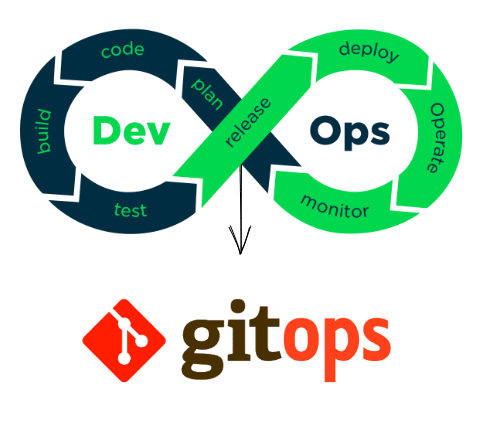
\includegraphics[width=0.60\linewidth]{assets/devops-gitops.png}
	\label{fig:devopsGitOps}	
\end{figure}

% develop new applications and services at high velocity

% reduce friction between engineering teams

% operations by interfacing with declarative state definitions stored in Git

\end{frame}

\begin{frame}
\frametitle{Problem Description}

\begin{figure}[h]
	\centering
	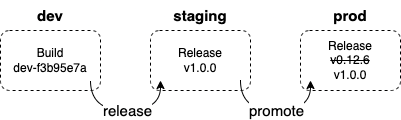
\includegraphics[width=.75\linewidth]{figures/release-promotion.drawio.png}
	\label{fig:releasePromotionProcess}	
\end{figure}

% promoting releases between multiple deployment environments

% Current GitOps tools (Flux, ArgoCD) do not provide an integrated solution

\end{frame}

\begin{frame}
\frametitle{Proposed Solution}

\begin{figure}[h]
	\centering
	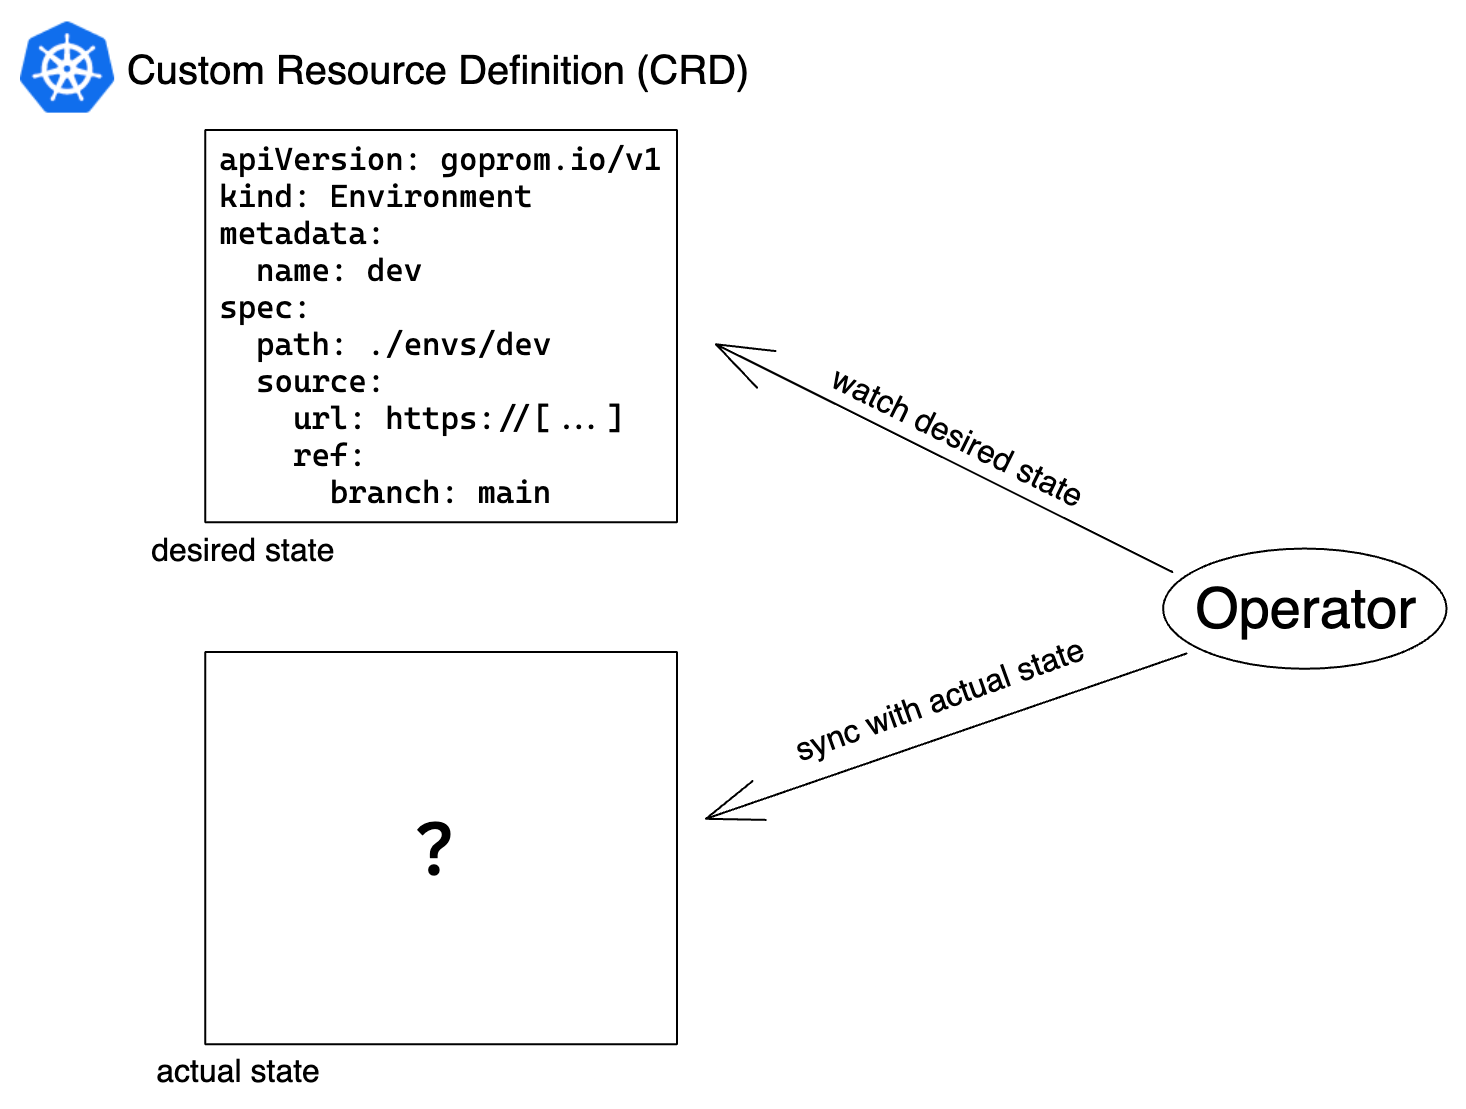
\includegraphics[width=.90\linewidth]{assets/crd-desired-actual-state-operator.png}
	\label{fig:crdDesiredActualStateOperator}	
\end{figure}

%standardised models for defining deployment environments and promotion processes

%application programming interface (API) extension for Kubernetes

%custom resource definitions

%allow users to define abstract representations of their environments and promotion processes

%Following the principles of GitOps, an operator would ensure the continuous reconciliation between the desired and the actual state of the resources.

\end{frame}

\begin{frame}
\frametitle{Big Picture}

\begin{figure}[h]
	\centering
	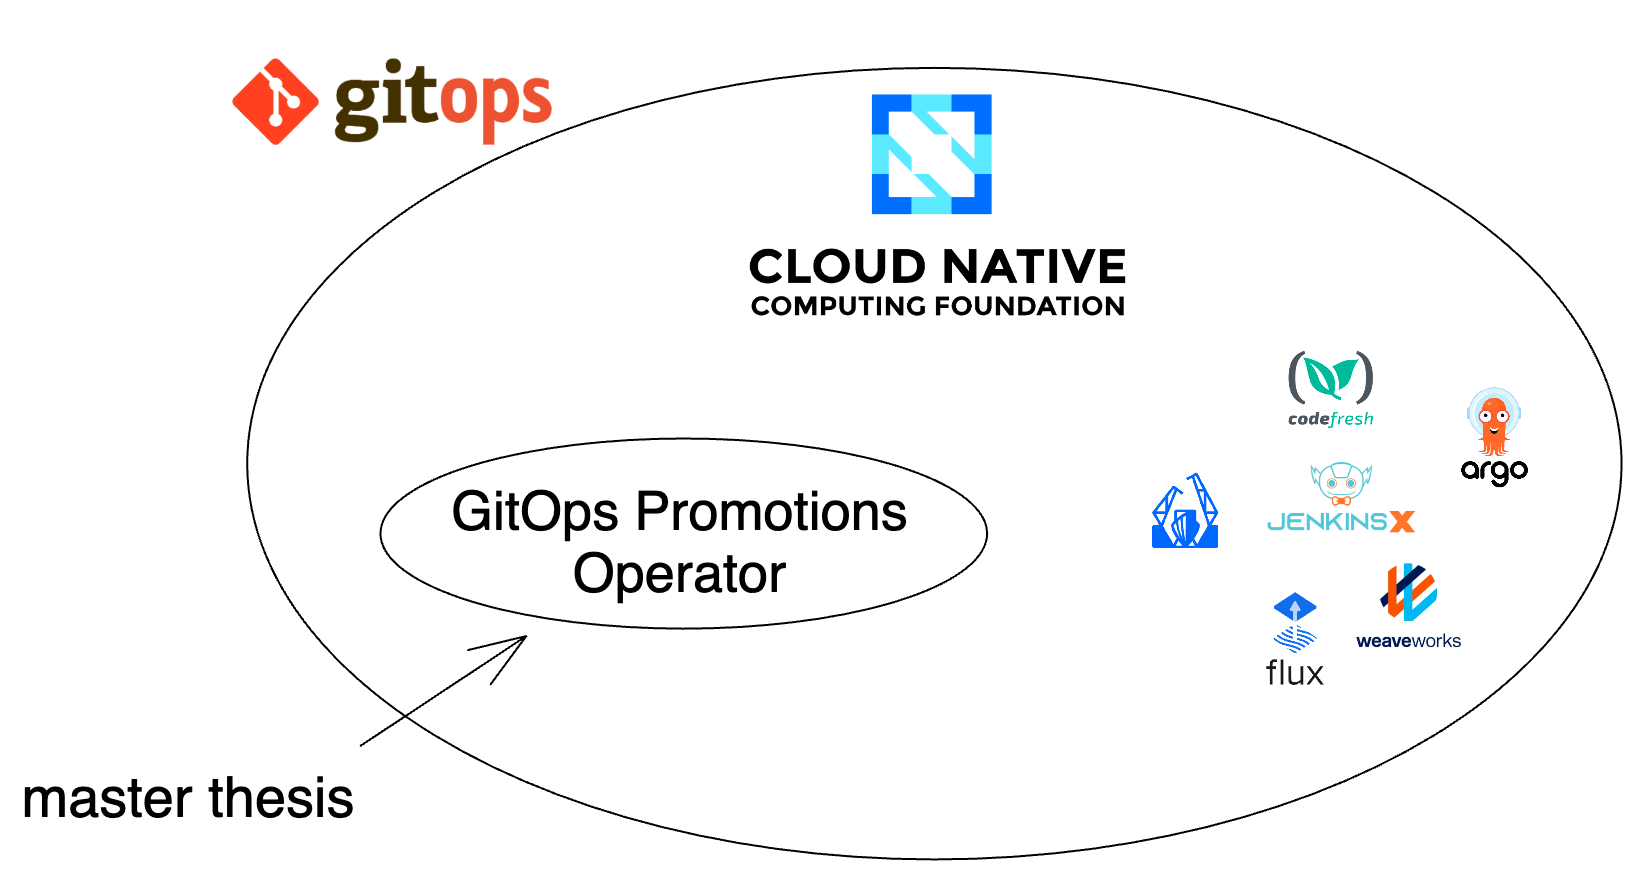
\includegraphics[width=1.00\linewidth]{assets/big-picture-release-promotion-operator-cncf-gitops.png}
	\label{fig:bigPictureReleasePromotionOperatorCncfGitops}	
\end{figure}

%The proposed solution of the problem should
%present a possible way of defining environments and promotion processes abstractly,
%onto which future work could build upon.
%
%Additionally the solution should
%provide a protoype of a toolkit,
%which could serve as an optional component
%in addition to existing tooling within the Cloud Native Computing Foundation (CNCF).
%
%Solving the problem of release promotion natively within the GitOps toolkit,
%would make the adoption of GitOps more appealing,
%especially for organisations, which have the need for many different environments.
%
%As a result
%this could generally accelerate the widespread use of GitOps
%and thus enable more organisations to develop higher quality software.

\end{frame}


\section{Related Work}

\begin{frame}
\frametitle{Related Work}

\begin{figure}[h]
	\centering
	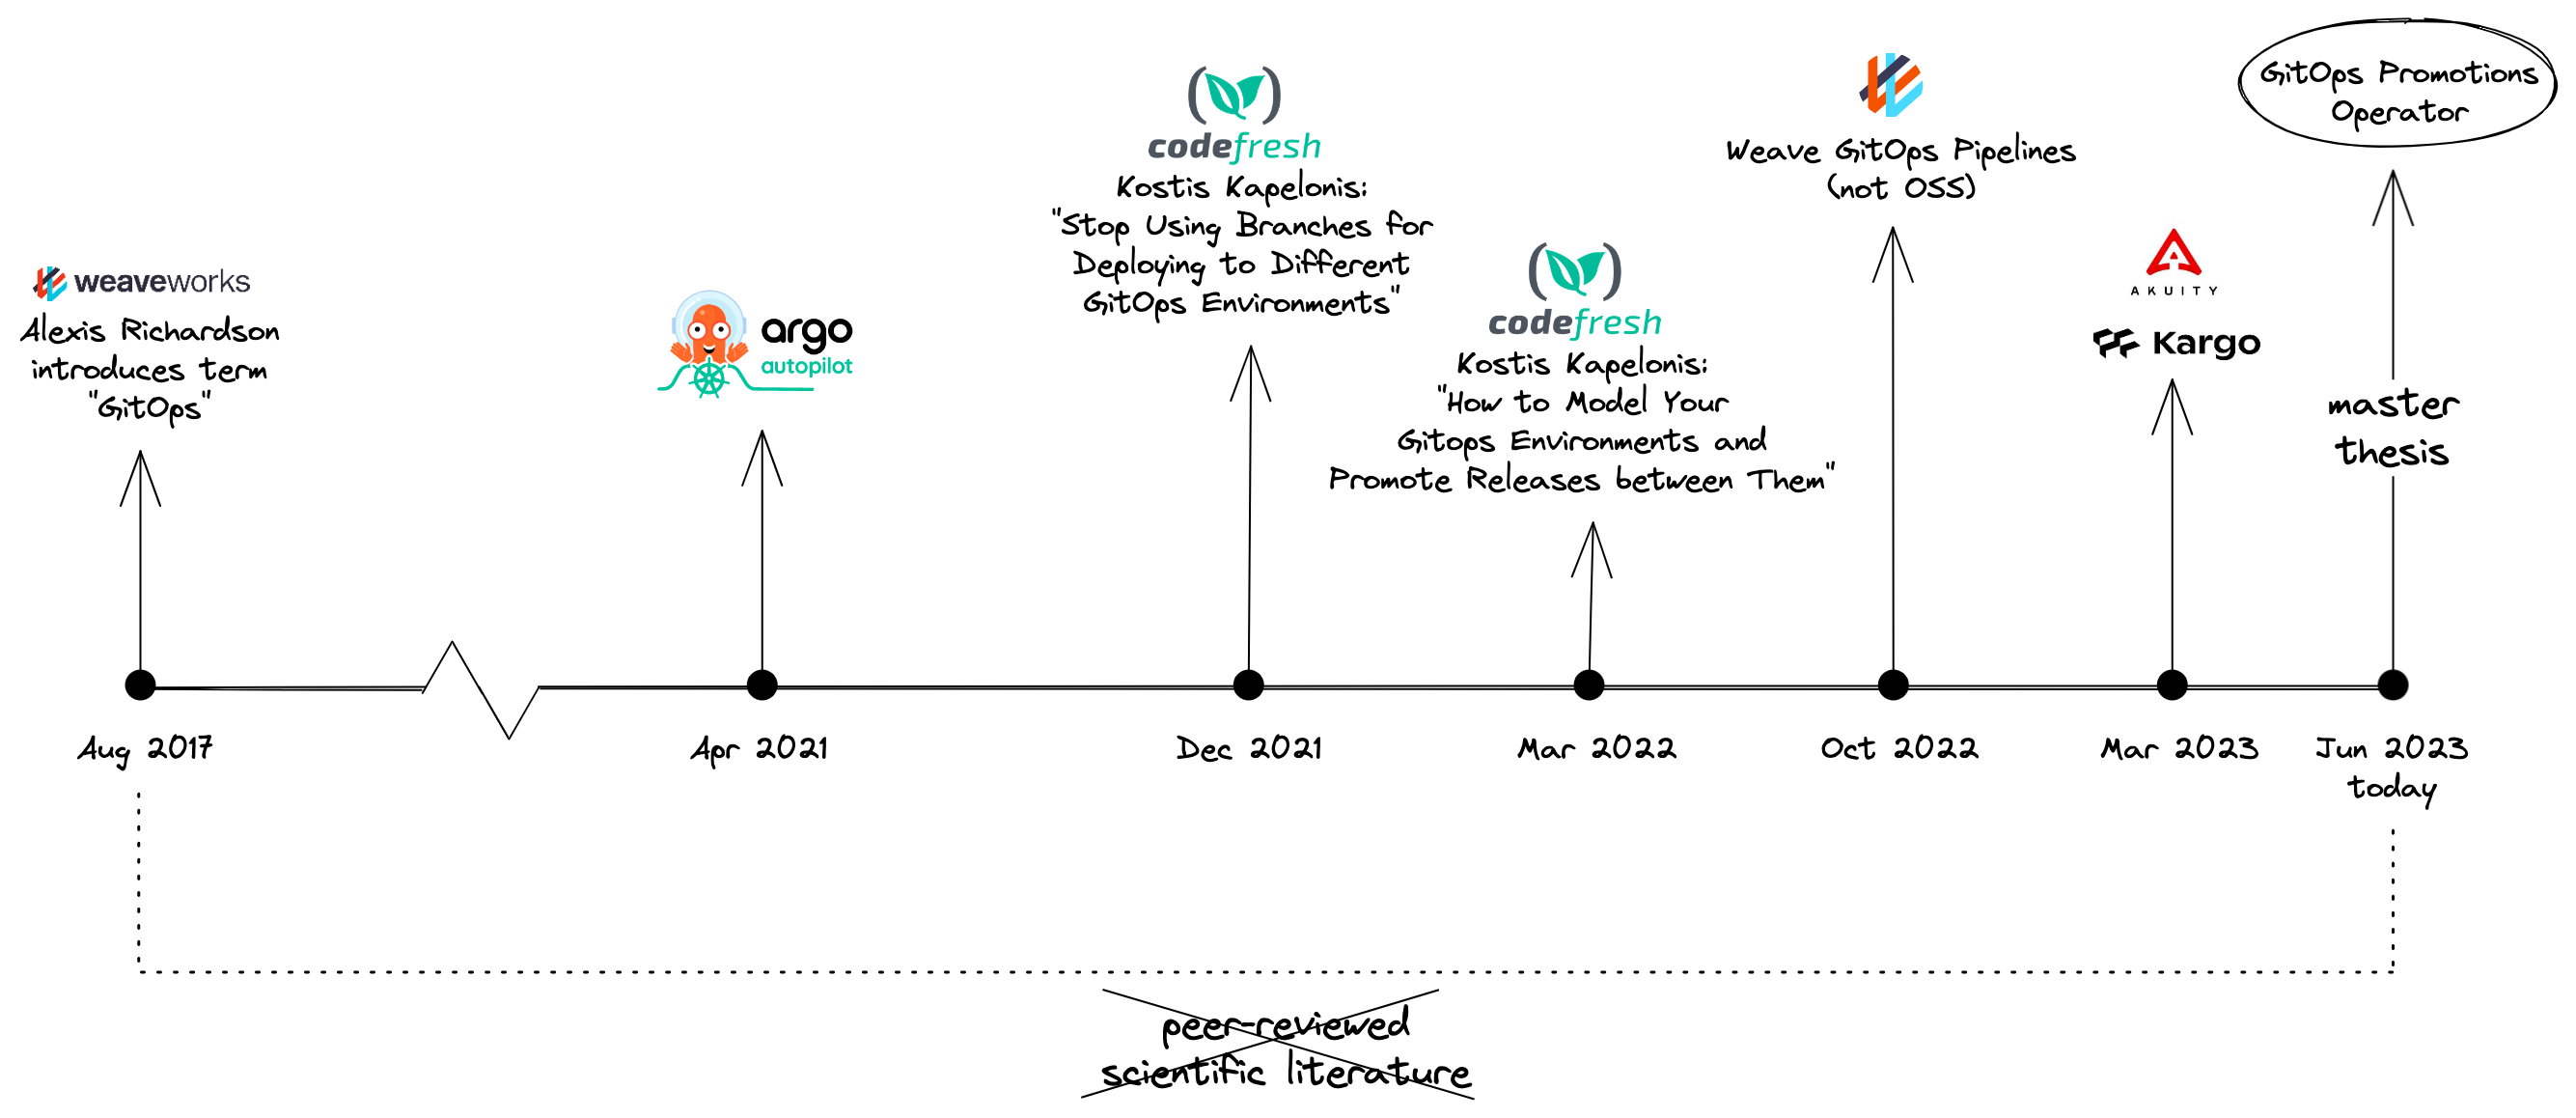
\includegraphics[width=1.0\linewidth]{assets/related-work-timeline-2017-2023-gitops.png}
	\label{fig:relatedWorkTimeline20172023gitops}	
\end{figure}

\end{frame}


\section{Research Questions}

\begin{frame}
\frametitle{Research Questions}

	\begin{itemize}
		\item How can the promotion of releases in GitOps environments be designed?
		\begin{itemize}
			\item What possibilities do existing tools offer for the promotion of releases with multiple deployment environments?
			\item How can deployment environments, as well as promotion processes be modeled abstractly?
			\item How can abstract modeling be used to implement a standardized solution for promoting releases?
		\end{itemize}
	\end{itemize}

\end{frame}


\section{Methodology}

\begin{frame}
	\frametitle{design science research in information systems \\
		\autocite{designScienceResearchMethodologyForInformationSystemsResearch}}
	
	\begin{figure}[h]
		\centering
		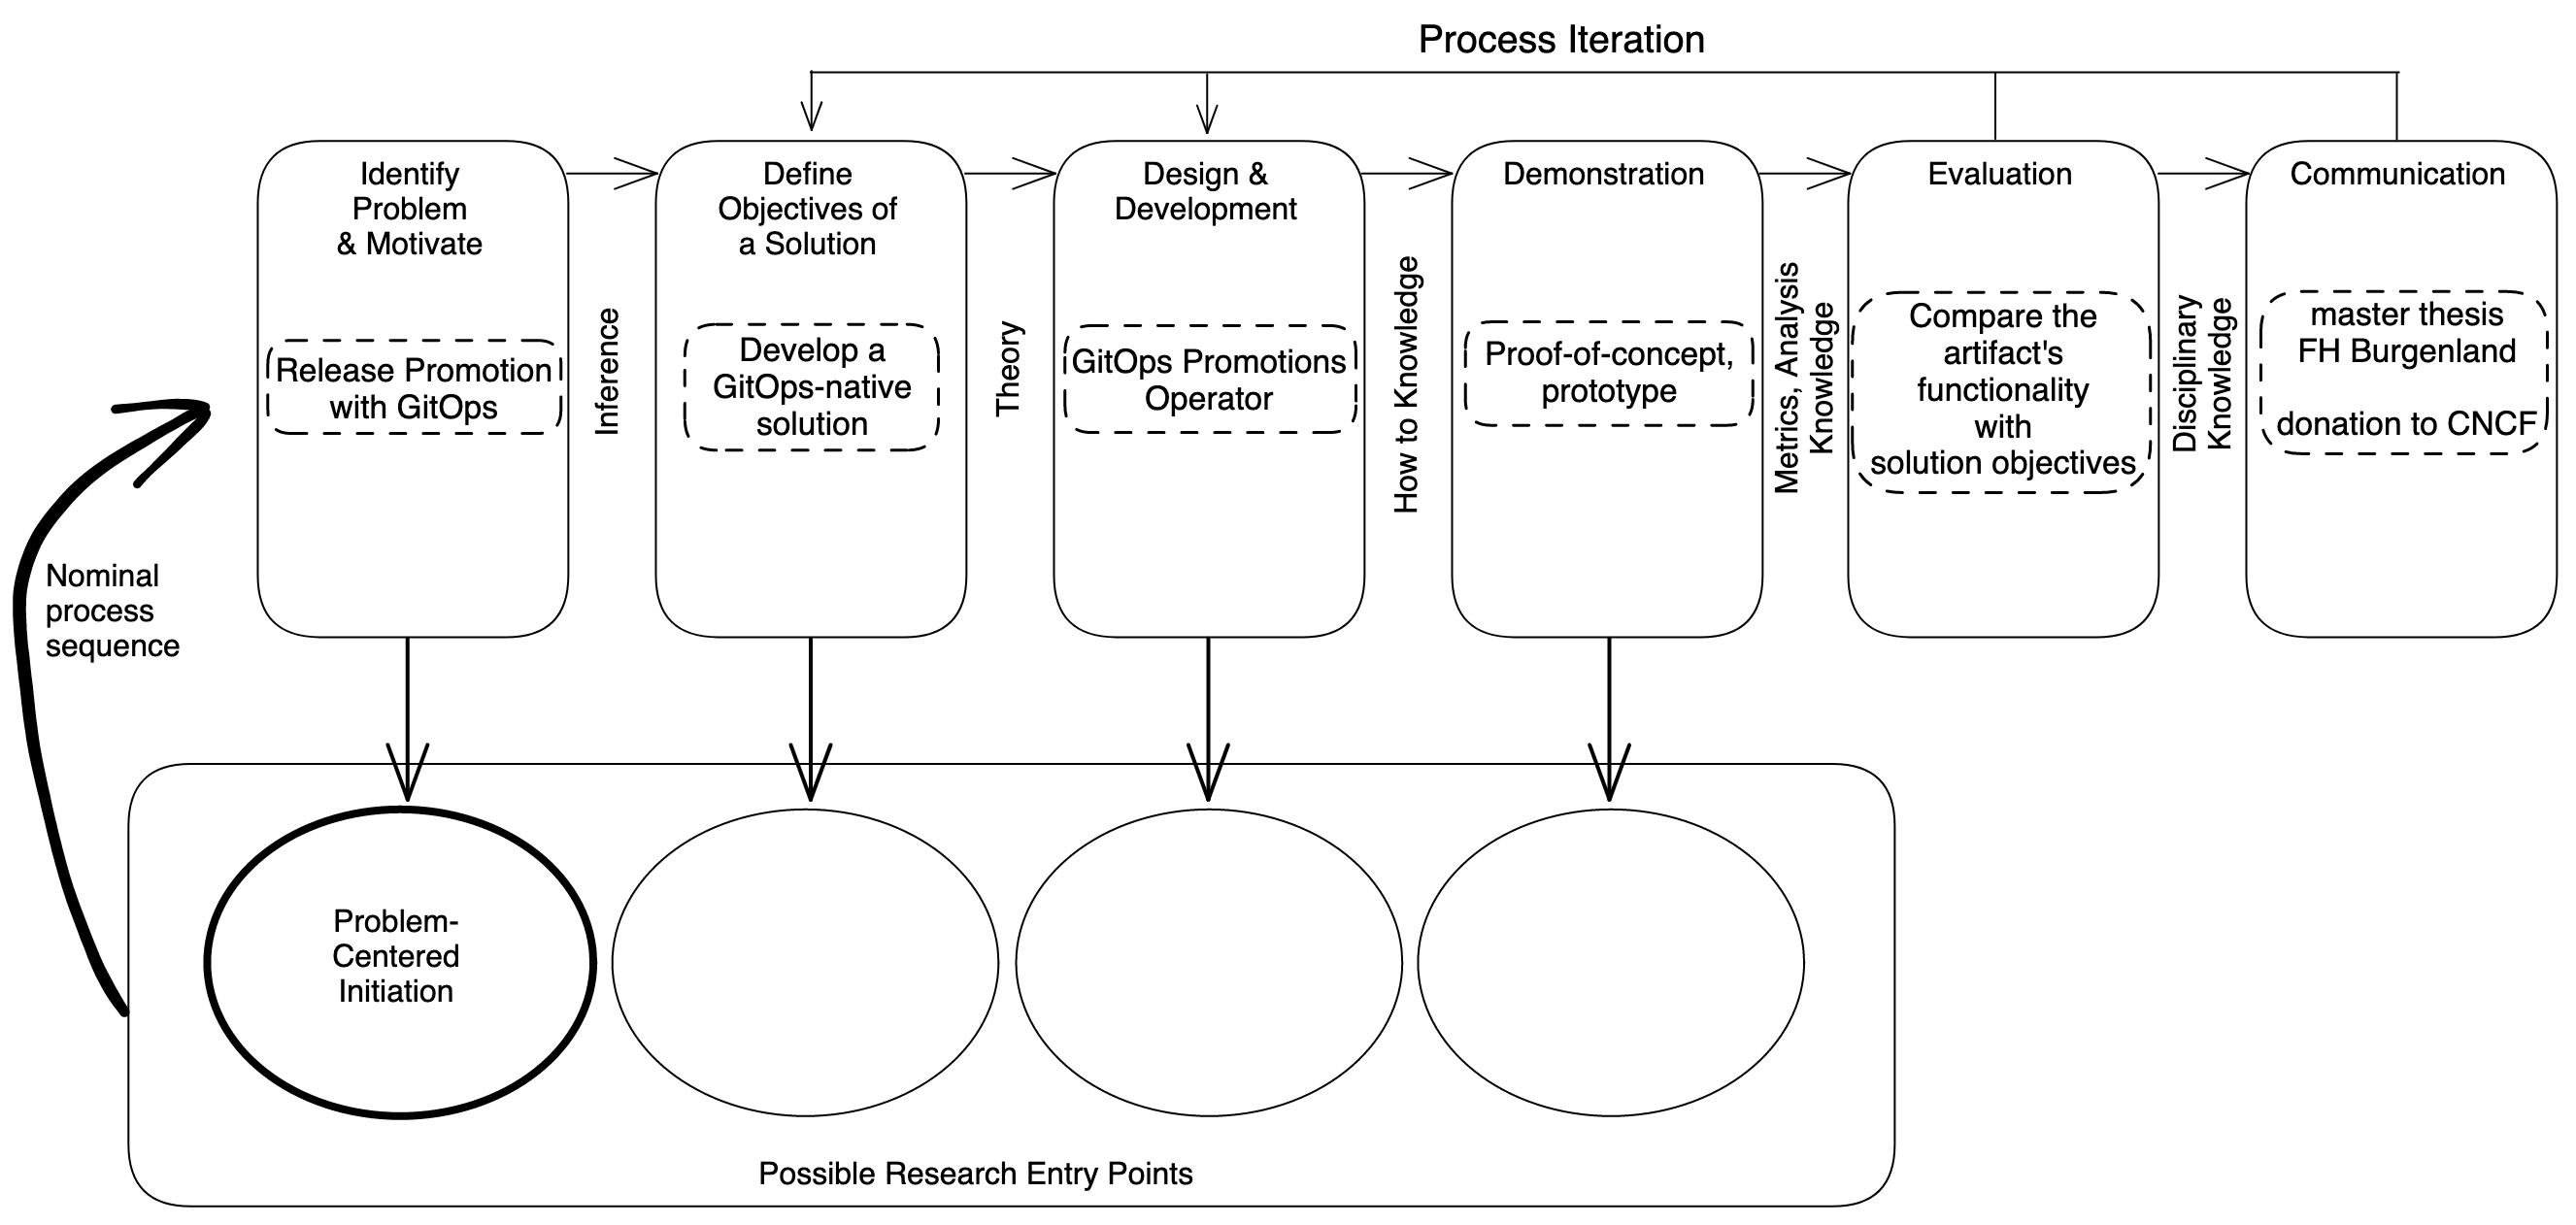
\includegraphics[width=1.00\linewidth]{figures/dsrm-process-release-promotion-gitops.png}
%		\caption{DSRM Process for this thesis.
			%		(\citeauthor{ref}, \citeyear{ref}).
%		}
%		\label{fig:dsrmProcessReleasePromotionGitOps}	
	\end{figure}

\end{frame}


\section{Results}

\begin{frame}
\frametitle{Results}

\begin{figure}[h]
	\centering
	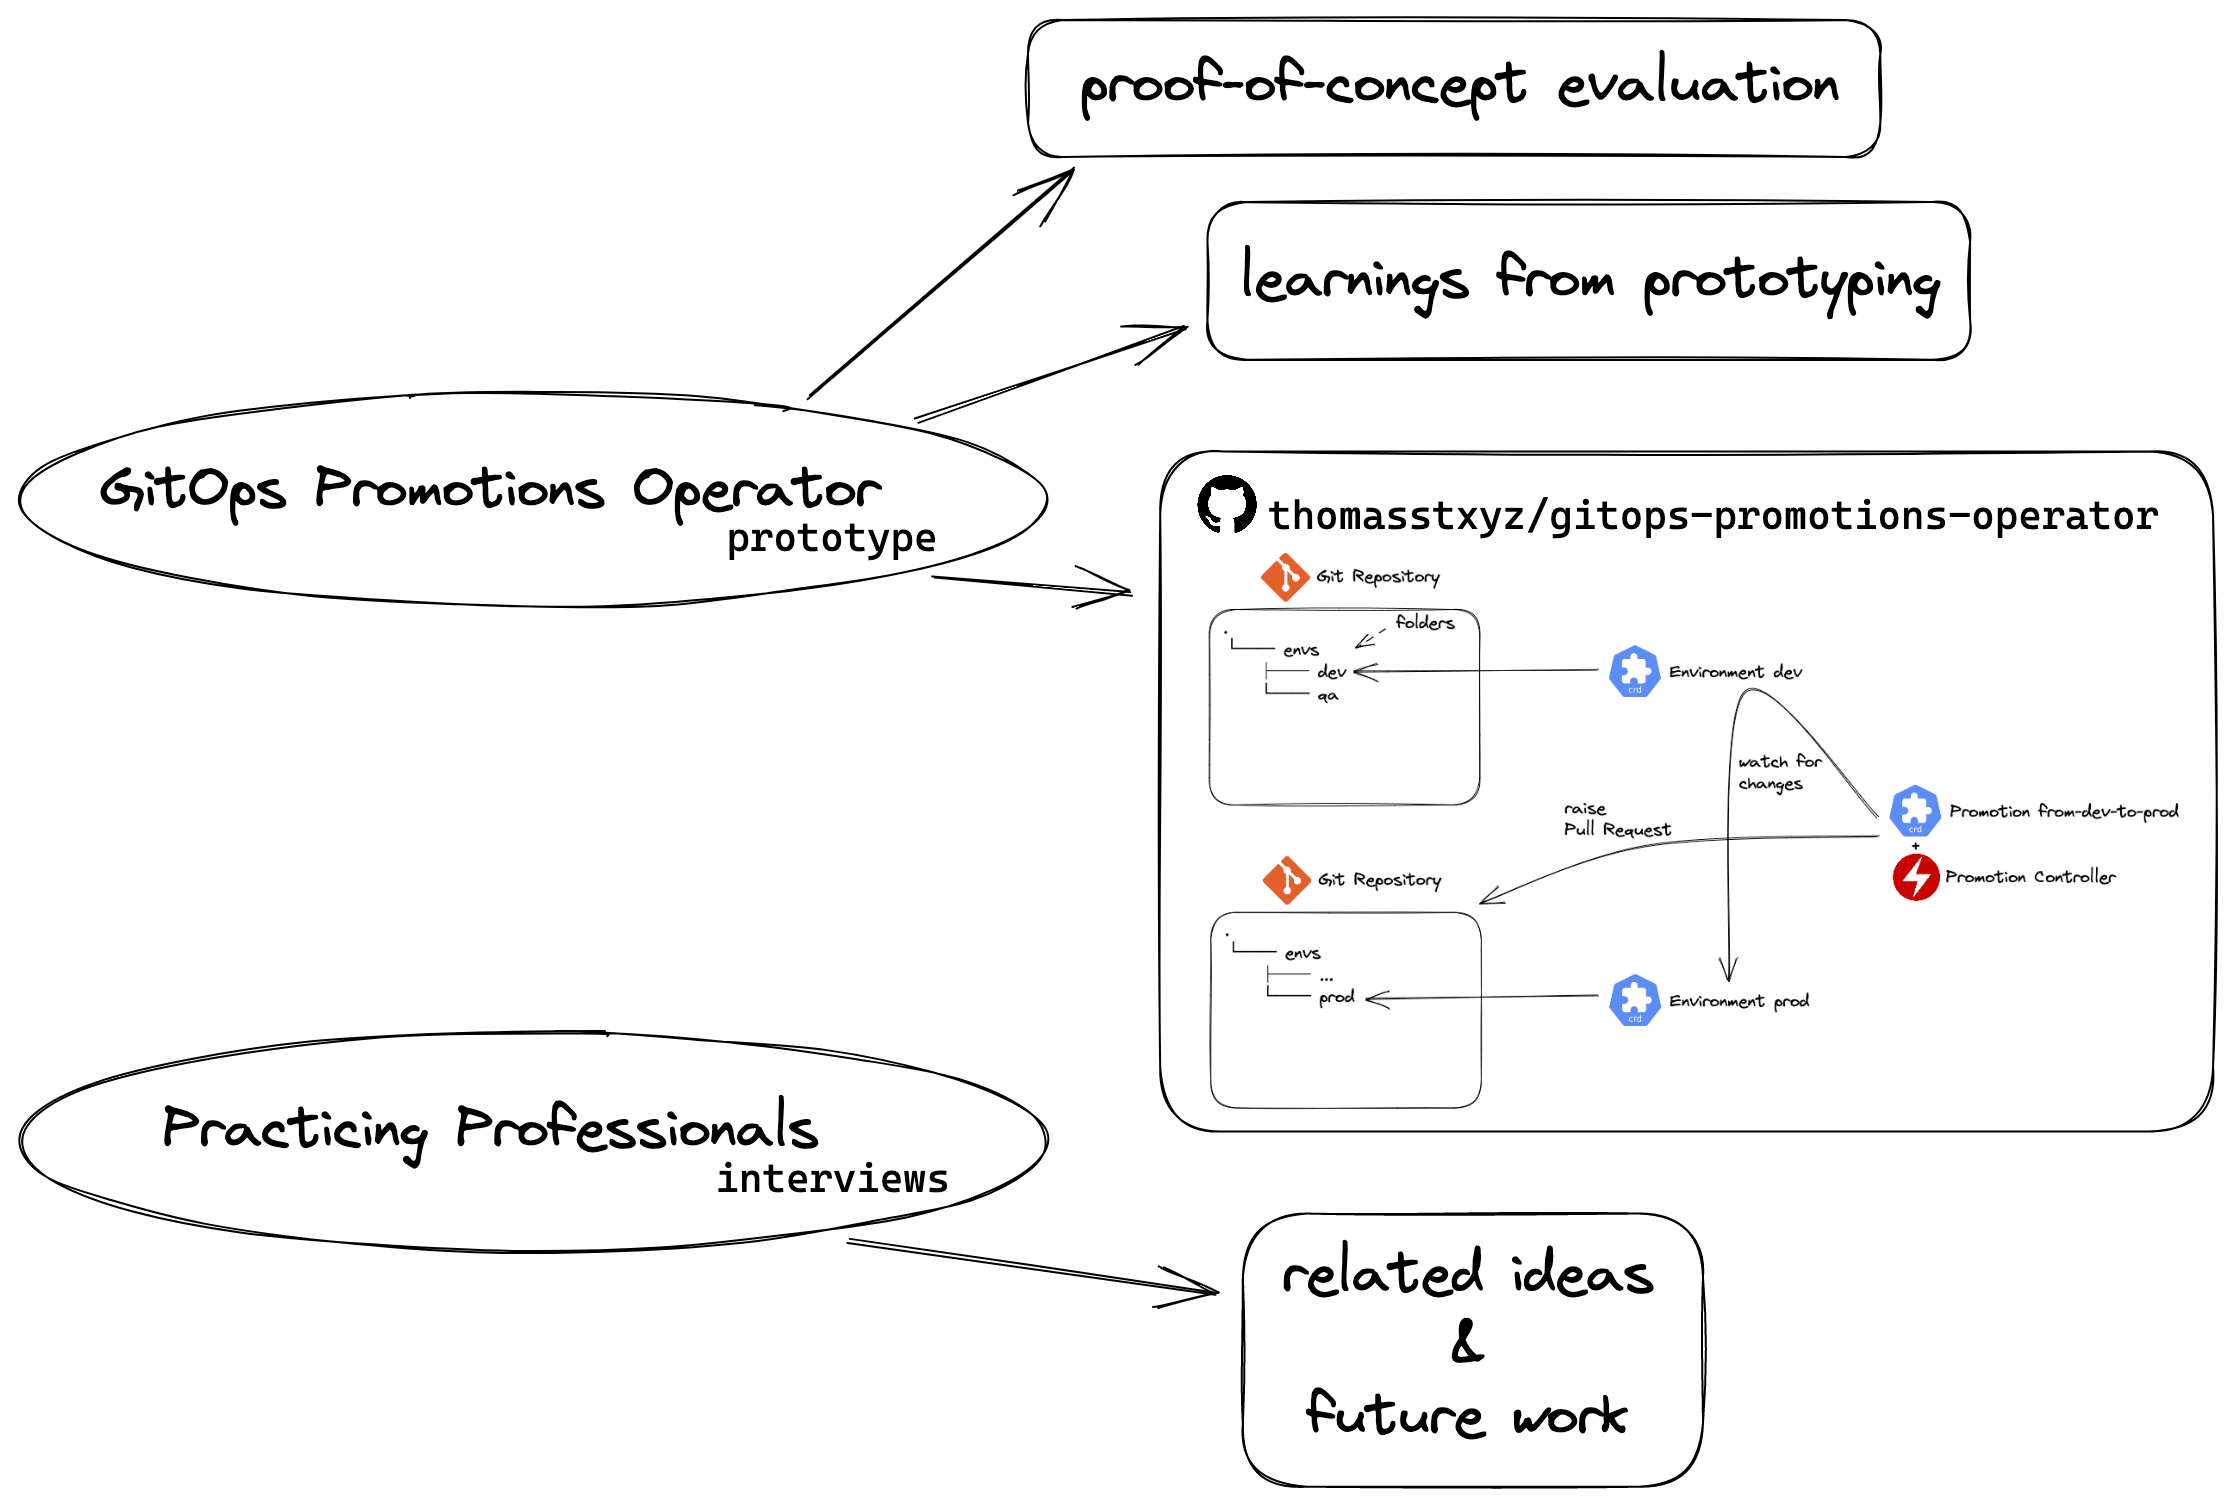
\includegraphics[width=1.0\linewidth]{assets/results-illustration-release-promotion-operator.png}
	\label{fig:resultsIllustrationReleasePromotionOperator}	
\end{figure}

%The overall goal of the thesis is to
%provide a solution to the problem of release promotion in GitOps environments.
%In this regard a prototype will be developed
%and its functionality demonstrated in a proof-of-concept evaluation.
%The goal for the prototype is to implement it as a modular extension to Kubernetes
%and existing GitOps tooling.
%By doing so, users can promote releases between multiple deployment environments
%following the GitOps principles.
%The main contribution of this thesis is a proof of concept for the developed prototype
%which can be used as an extension to the GitOps toolkit within the CNCF.

\end{frame}


\section{Conclusion and Future Work}

\begin{frame}
\frametitle{Conclusion}

\begin{figure}[h]
	\centering
	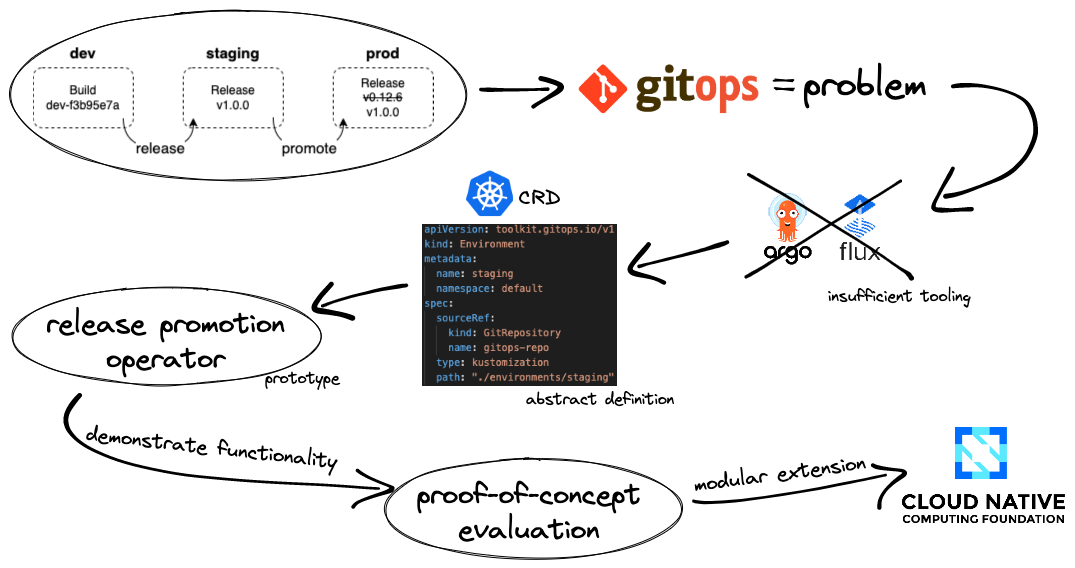
\includegraphics[width=1.0\linewidth]{assets/conclusion-gitops-thesis.png}
	\label{fig:conclusionGitopsThesis}	
\end{figure}

%The currently available GitOps tools
%do not provide an integrated solution to
%the problem of promoting releases between environments.
%This thesis aims at addressing the given problem.
%This is achieved by
%clearly defining the problem in distinct items,
%from which research objectives are then inferred.
%Following in designing and developing abstract models for
%environments and promotion processes;
%which are implemented in the produced artifact "release promotion operator".
%The artifact is demonstrated in a prototype serving as a proof-of-concept.
%Finally the research is evaluated by means of
%comparing the artifact's functionality with the solution objectives.
	
\end{frame}

\begin{frame}
\frametitle{Future Work}

\begin{figure}[h]
	\centering
	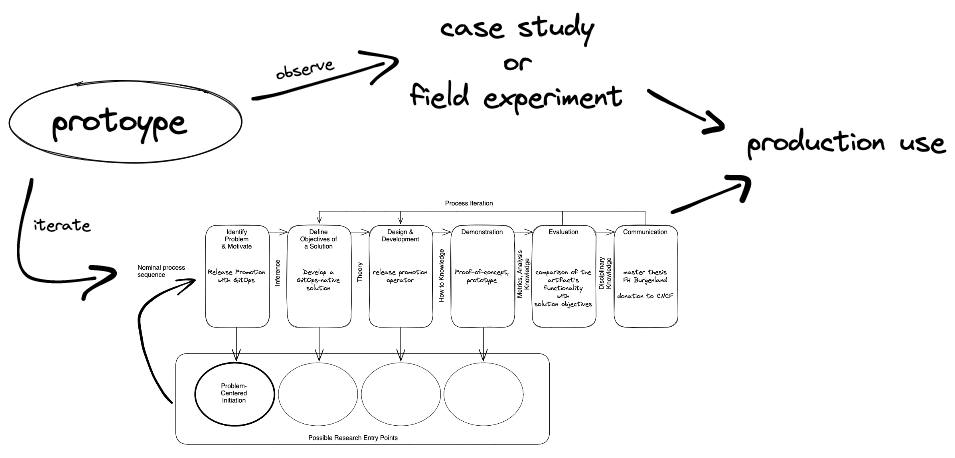
\includegraphics[width=1.0\linewidth]{assets/future-work-gitops-thesis.png}
	\label{fig:futureWorkGitopsThesis}	
\end{figure}

%The developed "release promotion operator" prototype should serve as
%a modular extension to Kubernetes and existing GitOps tooling within the CNCF.
%It should provide a more streamlined and GitOps-native approach
%to the process of release promotion.
%For subsequent research projects the use of the prototype could
%be observed in a case study or tested in a field experiment,
%and adapted in another iteration of the applied methodology process model.
%The main goal for future work is the extensive adaption of the prototype
%to enable use in production by organizations or other projects.

\end{frame}




%% columns in beamer
%\begin{frame}
%    \frametitle{Columns}
%    \begin{columns}
%        \column{.5\textwidth}
%        1 column
%        \column{.5\textwidth}
%        2 column
%    \end{columns}
%\end{frame}

\end{document}
